\section{Aufbau}
\label{sec:Aufbau}
\begin{figure}
	\centering
	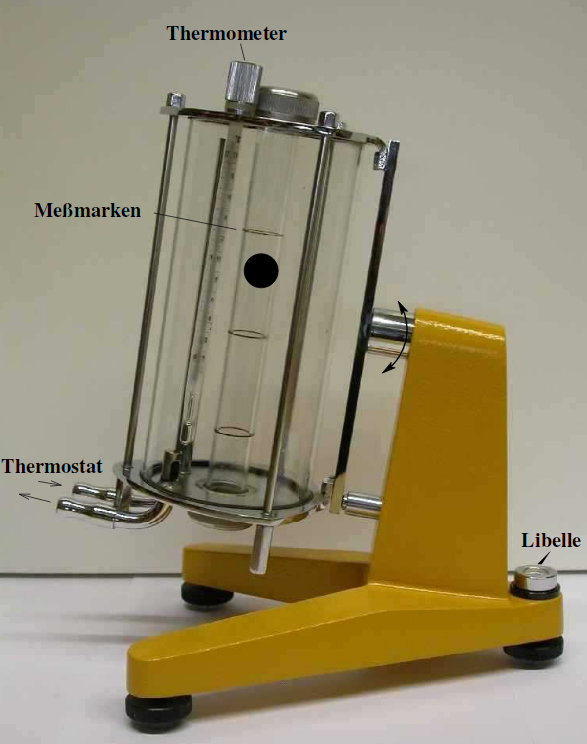
\includegraphics[width=\linewidth-100pt,height=\textheight-100pt,keepaspectratio]{content/Bilder/Hoeppler.png}
	\caption{Abbildung des Höppler-Viskosimeters \cite{V207}.}
	\label{fig:Aufbau2}
\end{figure}
Das Höppler-Viskosimeter besteht aus einer Glasröhre, welche mit der zu
untersuchenden Flüssigkeit gefüllt ist. In diese wird eine Kugel gesetzt, deren
Durchmesser nur geringfügig kleiner als der der Glasröhre ist. Damit die Kugel
nicht gegen die Wände der Fallröhre stößt, ist diese leicht geneigt. Das
Viskosimeter kann über eine Libelle ausgerichtet werden. Zur Messung
der Fallzeit sind Markierungen an der Röhre angebracht. Um die Temperaturabhängigkeit
der Viskosität zu untersuchen ist ein Wasserbad um die Fallröhre herum angebracht.
Diese kann über ein Thermostat kontrolliert erhitzt werden.
